\documentclass[11pt, aspectratio=169, compress]{beamer}
\usetheme[progressbar=frame title, numbering=fraction]{metropolis}      % Use metropolis theme 
\setbeamertemplate{section in toc}[sections numbered]
\setbeamertemplate{subsection in toc}[subsections numbered]
\useoutertheme[subsection=false]{miniframes}
\setbeamercolor{section in head/foot}{fg=white, bg=mDarkTeal}
\setbeamercolor{background canvas}{bg=white}
\setbeamerfont{section in head/foot}{series=\bfseries}

\usefonttheme[onlymath]{serif}
\usepackage{amsmath}
\usepackage{remreset}
\usepackage{ragged2e}
\usepackage{booktabs}
\usepackage{makecell}
\usepackage{float}
\usepackage{subfig}
\usepackage{tikz}
\usetikzlibrary{positioning,calc}
\usepackage[flushleft]{threeparttable}	% 3 part table 
\usepackage[justification=centering]{caption}
\captionsetup{skip=0pt}
\graphicspath{{./fig/}}

\makeatletter
\let\beamer@writeslidentry@miniframeson=\beamer@writeslidentry
\def\beamer@writeslidentry@miniframesoff{%
	\expandafter\beamer@ifempty\expandafter{\beamer@framestartpage}{}% does not happen normally
	{%else
		% removed \addtocontents commands
		\clearpage\beamer@notesactions%
	}
}
\newcommand*{\miniframeson}{\let\beamer@writeslidentry=\beamer@writeslidentry@miniframeson}
\newcommand*{\miniframesoff}{\let\beamer@writeslidentry=\beamer@writeslidentry@miniframesoff}
\beamer@compresstrue
\makeatother

%==============================================================
% Title Page
%==============================================================
%Information to be included in the title page:
\title{Interacciones sociales (continuación)}
\author{Rony Rodriguez-Ramírez} 
\institute{Economía Social y Humana | Grupo B018 \\Universidad Centroamericana}
\titlegraphic{\hfill
\includegraphics[height=1.5cm]{uca}}
\date{\today}
%==============================================================
\begin{document}
	
\begin{frame}[plain]
	\maketitle  
\end{frame}

%\begin{frame}{Outline}
%\tableofcontents[hideallsubsections]
%\end{frame}
%------------------------------------------------
\section{Comentarios y anuncios}
%-----------------------------------------------
\subsection{Comentarios y anuncios}
%-----------------------------------------------
\begin{frame}{Comentario y anuncios}
\begin{itemize}
	\item Ensayo grupal: Media - 9, Media General: 11.42
	\begin{itemize}
		\item Errores: Síndrome de la oracíon larga. 
		\item Separación entre sujeto y objeto. 
		\item Falta de cohesión y claridad. 
	\end{itemize}
\end{itemize}
\end{frame}
%------------------------------------------------
\section{Conley y Udry (2010)}
%------------------------------------------------
\subsection{Conley y Udry (2010)}
%------------------------------------------------
\begin{frame}{Aprendiendo sobre una tecnología: Piña en Ghana}
\textbf{Idea central:}
\begin{itemize}
	\item Investigar el papel del aprendizaje social en la difusión de una nueva tecnología agrícola. 
\end{itemize}
\textbf{Puntos a considerar:}
\begin{itemize}
	\item La transformaición de technología es fundamental para el proceso de desarrollo. 
	\item ¿Cómo se adaptan los agentes a nuevas tecnologías? ¿Qué tan rápido? 
\end{itemize}
\end{frame}
%------------------------------------------------
\begin{frame}{Aprendiendo sobre una tecnología: Piña en Gana}
\begin{itemize}
	\item Al considerar nuevas tecnologías se debe tomar en cuenta que se necesita invertir en aprendizaje. 
	\item Ahora, si hay muchas personas que adoptan la tecnología al mismo tiempo, el proceso de aprendizaje puede ser \textit{\textbf{social}.}
	\item La idea de aprendizaje social presente en: 
	\begin{itemize}
		\item Literatura de crecimiento endógeno.  
		\item Urbanización y crecimiento. 
		\item Externalidades. 
	\end{itemize}
\end{itemize}
\end{frame}
%------------------------------------------------
\begin{frame}{Contexto del artículo}
\begin{itemize}
	\item En los 90s, existía un sistema establecido de maíz y cassava (yuca) intercaldo que comenzó a ser transformado por la producción intesiva de piña para exportar. 
	\item Involvía la adopción de nuevas tecnologías: fertilizador y otros químicos. 
	\item La pregunta entonces es: 
	\begin{itemize}
		\item ¿Cuál fue el rol del aprendizaje social en este proceso? 
	\end{itemize}
\end{itemize}	
\end{frame}
%------------------------------------------------
\begin{frame}{Aprendizaje social}
	\begin{itemize}
		\item Por un lado, medir aprendizaje social es difícil: 
		\begin{enumerate}
			\item El set de vecinos de los cuales se puede aprender es difícil de difinir. 
			\item Distinguir ese aprendizaje de otros fenomenos es problemático. 
		\end{enumerate}
		\item Por otro lado, información sobre interconecciones es típicamente no disponible. 
	\end{itemize}	
\end{frame}
%------------------------------------------------
\begin{frame}{Aprendizaje social}
	Ventajes del estudio: 
	\begin{itemize}
		\item Los autores recolectaron información sobre quiénes conocen y hablan sobre agricultura para definir enlaces de información. 
		\item Los datos contienen: 
		\begin{itemize}
			\item Detalles geográficos, información sobre el suelo, crédito, relación familiar para controlar por estos factores. 
		\end{itemize}
	\end{itemize}
\end{frame}
%------------------------------------------------
\begin{frame}{Problema general en los estudios de interacciones sociales}
\begin{itemize}
	\item Principal preocupación: 
	\begin{itemize}
		\item Inferir si el comportamiento de un individuo está influenciado por las características de las personas en su vecindario. 
	\end{itemize}
	\item Para lograr solucionar este problema: 
	\begin{itemize}
		\item La identificación de los efectos de aprendizaje se basa en el uso del tiempo específico de las plantaciones para identificar oportunidades para la transmisión de información. 
		\item Inclusión de la información del vecino. 
	\end{itemize}
\end{itemize}
\end{frame}
%------------------------------------------------
\begin{frame}{Enlaces de información}
	\begin{itemize}
		\item Proximidad espacial está correlacionada con la presencia de links de informaciónpero no es el determinante único. 
		\item También ocurre en largas distancias como en cortas. 
		\item Con las distancias mayores se permite distinguir el impacto de la información de la correlación espacial. 
		\item Punto importante: cruce entre géneros es raro y posiblemente correlacionada solo con familia, clan, etc. 
	\end{itemize}
\end{frame}
%------------------------------------------------
\begin{frame}{Inputs y outputs}
	\begin{itemize}
		\item Conley y Udry (2010) se enfocaron en la intensidad de los inputs que se ocuparon en la producción de piña: 
		\begin{enumerate}
			\item Fertilizador. 
			\item Trabajo. 
		\end{enumerate}
	\end{itemize}
\end{frame}
%------------------------------------------------
\begin{frame}{Principales resultados}
	\begin{itemize}
		\item Aprendizaje social es importante en la difusión de conocimiento.
		\item Los agricultores cambian los niveles de sus inputs al conocer o recibir malas noticias sobre la rentabilidad del uso del nivel anterior de sus inputs.
		\item Menos probable que cambien cuando observan malas noticias sobre la rentabilidad de niveles de otros inputs.
		\item Agriculturos incrementan (disminuyen) el uso de inputs cuando un vecino registra una ganancia (perdida) mayor a la esperada. 
		\item Ajuste en inputs, relación de agricultores novatos y veteranos.
	\end{itemize}
\end{frame}
%------------------------------------------------
%------------------------------------------------
\section{Bandiera, Barankay, y Rasul (2005)}
%------------------------------------------------
\subsection{Bandiera, Barankay, y Rasul (2005)}
%------------------------------------------------
\begin{frame}{Idea general}
	\begin{itemize}
		\item Comparar la preferencias sociales de los trabajadores bajo incentivos relativos donde se impone una externalidad negativa en los demás, con la productividad por pieza donde no se impone. 
	\end{itemize}
\end{frame}
%------------------------------------------------
\begin{frame}{Preferencias sociales: evidencia previa e importancia} 
\begin{itemize}
	\item Evidencia sobre como los individuos toman en cuento el efecto de sus acciones en otros pero ``en el laboratorio.''
	\item Gran relevancia:  
	\begin{itemize}
		\item La productividad de los trabajadores dentro de ciertos esquemas de incentivos, como evaluación de su desempeño y pago en equipo, depende crucialmente en como las personas internalizan sus acciones. 
	\end{itemize} 
\end{itemize}
\end{frame}
%------------------------------------------------
\begin{frame}{Preferencias sociales: evidencia previa e importancia} 
Bandiera et al. (2005) estudian esto en una granja en UK: 
\begin{itemize}
	\item La granja primero paga a sus emepleados de acuerdo a une esquema relativo de incentivos y luego cambia a pago por destajo. 
	\begin{itemize}
		\item Comparan productividad dentro de los dos esquemas. 
	\end{itemize}
	\item En los incentivos relativos, se paga de acuerdo a la proporción de la productividad promedio. 
	\item Dentro del otro esquema se paga de acuerdo a la productividad individual. 
\end{itemize}
\end{frame}
%------------------------------------------------
\begin{frame}{Datos}
Cautro elementos para identificar el efecto causal: 
\begin{enumerate}
	\item Observan la productividad diaria de los mismo trabajadores antes y después de la introducción del pago por destajo. 
	\item Los mismo trabajadores enfrentan ambiente laboral identico excepto por los cambios en los incentivos. 
	\item El grupo de co-trabajadores con los cuales un individuo trabaja cambia diariamente. 
	\item Observan a un subgrupo (submuestra) de los mismo trabajadores usando una tecnología alternativa que no monitorio a sus co-trabajadores. 
\end{enumerate}
\end{frame}
%------------------------------------------------
\begin{frame}{Resultados generales}
\begin{itemize}
	\item El cambio de incentivos tiene un impacto significativo y permanente en la productividad: 
	\begin{itemize}
		\item Incremente de por lo menos 50 por ciento en la productividad al moverse de un esquema de incentivos relativos a destajo. 
		\item Los trabajadores no ignoran la externalidad negativa que imponen a sus compañeros. 
		\item Sin embargo, el cambio no es tan grande para decir que los trabajadores internalizan \textit{completamente} la externalidad negativa. 
		\item Productividad es mejor cuando las trabajadores se pueden monitorear entre si (caso de colusión). 
	\end{itemize}
\end{itemize}
\end{frame}
%------------------------------------------------
\begin{frame}{Resultados generales}
\begin{figure}[htb]
	\centering
	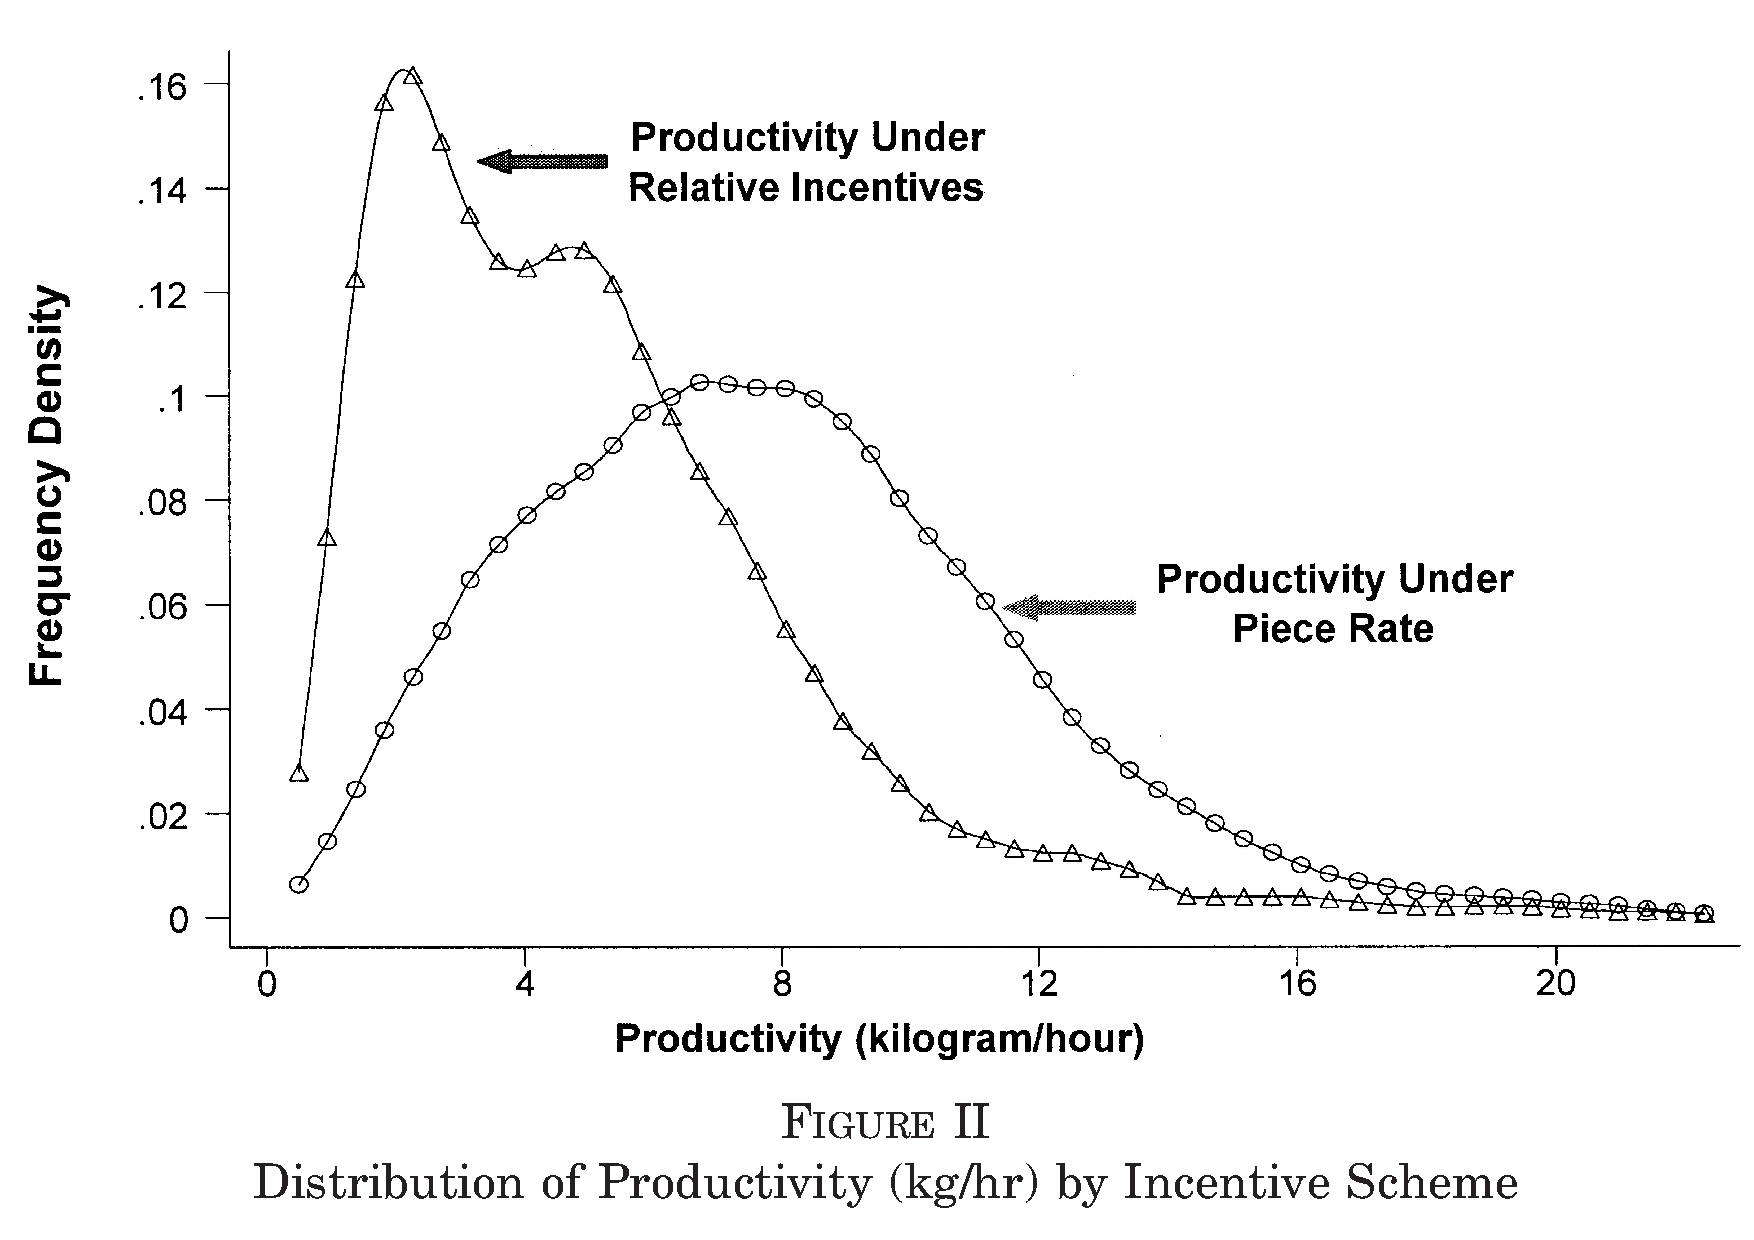
\includegraphics[width=.7\textwidth]{fig1}
\end{figure}
\end{frame}
%------------------------------------------------
\begin{frame}{Conclusiones}
Evidencia de cómo el comportamiento es explicado por las preferencias sociales de las personas. 
\begin{itemize}
	\item El hallazgo de que los trabajadores colocan un peso positivo en las recompensas de sus compañeros de trabajo también indica que las tarifas por pieza podrían no ser óptimas en este contexto. 
	\item Entender las preferencias de los trabajadores es fundamental para encontrar óptimos esquemas de incentivos. 
\end{itemize}
\end{frame}

%==============================================================
% END
%==============================================================
\miniframesoff 	
\begin{frame}[plain, standout]
Nos vemos la siguiente semana. 
\end{frame}

\end{document}		
